\section{Results}

\label{sec:results}


\subsection{Functional system}

The metrics for the evaluation of the functional BLEATS system are two
dimensional. This section will first evaluate and describe the evaluation of
the functional BLEATS system in terms of the desired characteristics and
functions of an attendance tracking system and will then subjectively evaluate
the functional system’s areas of improvement.

\subsubsection{Desired Characteristics and Functions}

The BLEATS system was developed with the desired characteristics and functions
of an attendance tracking system in mind. The five characteristics are speed,
deployment ease, authentication accuracy, reliability, and scale. The three
desired functions are recording identity, matching location, and noting the
time. These metrics were determined to be valid metrics for evaluating the
functional BLEATS system due to the characteristics being metrics that similar
solutions strive to achieve as well as the functions being a standard
definition for the functions of an attendance tracking solution.

In terms of speed, the functional BLEATS system embodies this characteristic by
utilizing BLE beacon communication. By doing so, no association between the
instructor device and the student device is ever necessary. The student device
communicates with the instructor device exclusively through indiscriminate
beacons and the instructor device communicates with the student device through
one way SMS message requiring no association. As such, the overhead of
initiating and maintaining an association is negated and the speed
characteristic is considered. In terms of deployment ease, the functional
BLEATS system contains this characteristic as it is implemented with the vision
in mind that it can be easily deployed to any mobile phone with BLE capability.
In terms of authentication accuracy, the functional BLEATS system uses dual
authentication with consideration for many approaches of dual authentication to
ensure identity. This provides for a higher level of confidence in identity
than an exclusively single factor authentication solution. However, it is
recognized that there are always methods to improve upon authentication
accuracy but many of these methods come at the cost of increased complexity or
reduced user space. For example, three factor authentication would increase
authentication accuracy but would greatly increase complexity and possibly
required user interaction. Also, biometrics as a form of second factor
authentication would likely improve the authentication accuracy but there are
less mobile phones available with biometric capabilities than with SMS
capabilities. 

One solution of interest that would provide an increase in authentication
accuracy without much added complexity is a form of threshold cryptography. In
threshold cryptography, multiple parties (in our environment, multiple
students) share the responsibility for cryptographic
functions~\cite{zhou1999securing}. In threshold cryptography, multiple parties
share a cryptographic key and then one party requires the collaboration of
other parties to perform cryptographic actions. An adaptation of this protocol
to the current functional BLEATS system would be an encryption of the one time
code sent to each student. If the decrypting key were shared via threshold
cryptography amongst students in the classroom, none of the benefits of the
current SMS dual authentication would be lost but the student would be required
to be near their peers in the classroom to decrypt the code. This would
increase authentication accuracy by ensuring that all of the students needed to
decrypt the code were in the classroom as they would need to share their keys
quickly before the timeout mechanism. This sharing could be done through BLE
communication and without user interaction and would add a back-end, proximity
based authentication method without added complexity to the user. This should
be implemented in a future version of the functional BLEATS implementation.

In terms of reliability, the functional BLEATS system uses a forgiveness
mechanism through an updated “attempts” count in an authentication database to
give the user multiple chances to respond correctly to a one time code. This
makes considerations for an unreliable environment in which a student may not
respond be able to respond to a one time code message in less than the timeout
time. 

In terms of scale, the functional BLEATS system is untested. The current
functional BLEATS system has only been tested in practice between one student
device and one instructor device. This is a future source of evaluation for
this system.

In terms of the function of recording identity, the functional BLEATS system
uses dual factor authentication to ensure the identity of a student that is
checking in to the attendance system while using a database to be able to look
up the student and record their identity. In terms of the function of matching
location, the use of BLE beaconing supports the student being present in the
classroom in order to check in to the attendance tracking instructor device. In
terms of noting of time, the functional BLEATS system leverages a timeout
mechanism to ensure that the student checking in to the attendance system is
doing so at the time of the attendance query.

\subsubsection{Areas of Improvement}

A subjective evaluation resulting in reporting room for improvement was
determined to be a necessary and valid evaluation tool for the functional
BLEATS system due to the BLEATS system being a user application at its core
with a need for user’s to subjective enjoy using it and feel confident in its
efficacy. The first area of improvement in the current system is that the
BLEATS student side system should be implemented on a mobile phone instead of a
Raspberry Pi/ mobile phone tandem. This would support the vision of the
solution as a solution that could be used with students’ previously owned
mobile devices. A second area of improvement for the BLEATS system is that the
system is currently scoped to one student and one instructor device. The BLEATS
system needs to be implemented for and tested for a scale consistent with that
of a large university classroom. Currently, the system is statically coded in
certain places (such as with the phone numbers) to support only one student. A
third area of improvement for the BLEATS system is in increasing the
authentication accuracy without added complexity and/ or user interaction. The
threshold cryptography scheme described in the previous evaluation section
“Desired Characteristics and Functions” is one possibility for improving on
this area. Another possibility for improvement in this area is in insight
gained from current, in use wireless sensor network authentication schemes such
as those described in~\cite{kumari2014cryptanalysis}. Wireless sensor networks
mirror many of the concerns of the BLEATS solutions as both require one way
communication to a central server from nodes in a specific area and the modern
authentication schemes of wireless sensor networks may provide insight that can
be used in BLEATS authentication. A fourth area of improvement is that the
BLEATS system should require no interaction from the student and should be
fully automated from both the instructor and student devices. A fifth area of
improvement would be in power management. Currently, the system requires the
student device’s BLE be turned on at all times. If the BLE were turned on only
when needed for transmitting the two BLE beacons and then turned off following
transmission, power consumption could be improved for the BLEATS system. A
sixth and final area for improvement for the functional BLEATS system is a more
refined timeout mechanism. The current timeout mechanism on the instructor
machine only determines a timeout of a student’s code once it has received a
BLE beacon from the student with a code. If the student does not attempt to
send a code, then the instructor machine will not generate a new code and send
it again to the student. A secondary timeout event that sends a new code
without student prompting could improve upon the BLEATS implementation.

\subsection{Simulation Results}

\subsubsection{Transmission Range}

\begin{figure} \centering
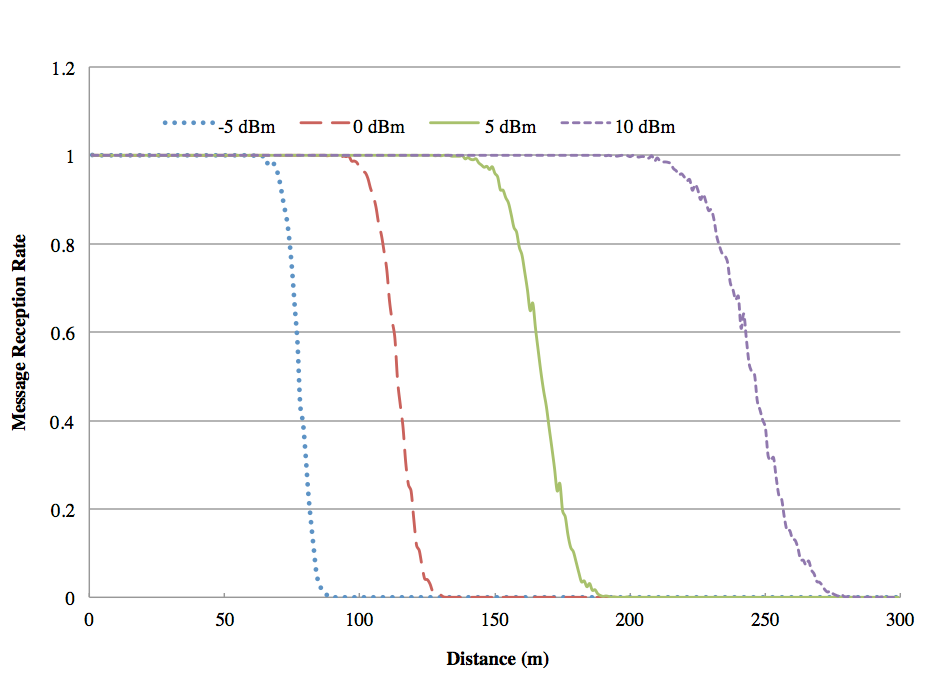
\includegraphics[width=\columnwidth]{figures/distance-error.png}
\caption{Reception success rate across power levels measured over 1000 messages for a single beacon}
\label{fig:distance-error} \end{figure}

Following our initial approach plan, we first evaluate the distance at which
BLE can operate for a single node. Bluetooth can operate from -20 to 10 dBm,
and we characterize distance performance at different transmission power levels
within that range (Figure~\ref{fig:distance-error}). We see that the maximum
range for BLE transmission is around 200 meters before messages start to drop.
In a typical real-world environment, however, there is abundant interference
from other wireless protocols that use the same frequency band, namely 802.11
WiFi, which would drastically reduce the reliable transmission range.
Additionally, in the BLEATS system, battery-powered mobile devices act as the
transmitters, so we pick 0 dBm as the baseline transmission power to use for
subsequent simulations. 0 dBm provides a balance between acceptable optimal range (100m) and
reduced power consumption.

\subsubsection{Topology and Device Density}

\begin{figure} \centering
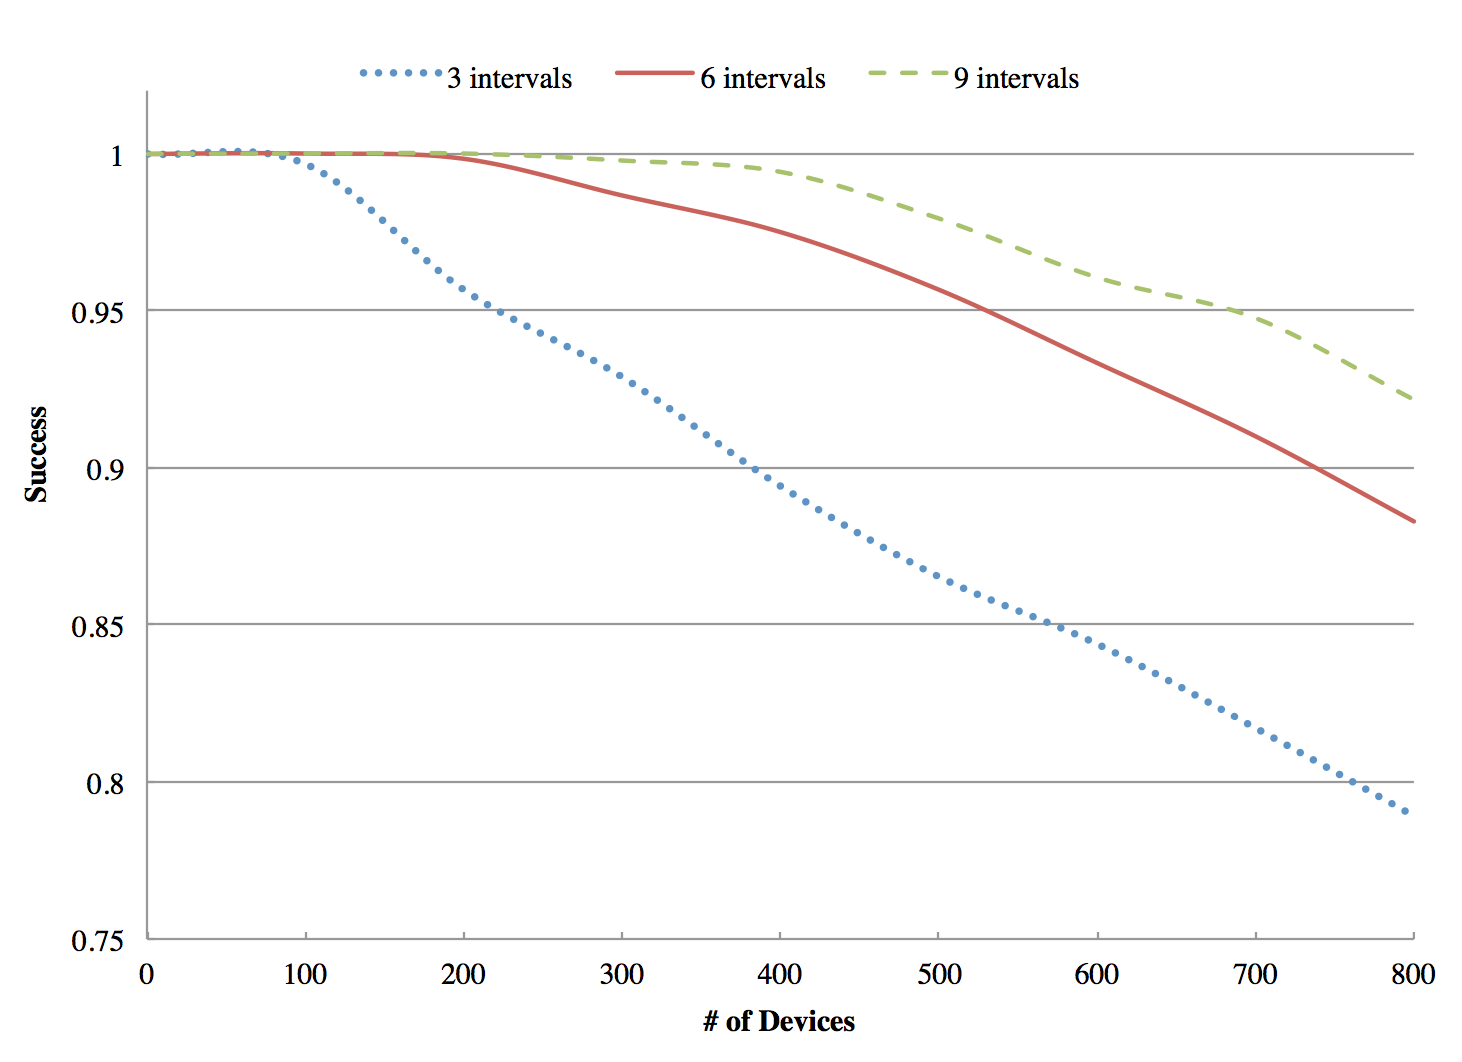
\includegraphics[width=\columnwidth]{figures/base-topo-error.png}
\caption{Transmission success rate across all intervals for baseline topology, all devices co-located 10m from the receiver.}
\label{fig:base-topo-error} \end{figure}

We evaluate the transmission success rate of 100 millisecond intervals over 3,
6, and 9 interval-long scans for a baseline topology of a single receiver and
all beacon nodes co-located a single point 10 meters away
(Figure~\ref{fig:base-topo-error}). This simulation is useful for observing
the reliability characteristics of BLEATS with respect to scan length. For this
simulation, the success percentage is determined by the number of nodes that
had at least one successful message transmission during the total scan length.
Based upon this definition, reliable transmission essentially requires 100\%
success. We find that for 3-interval scans, even 100 nodes leads to unreliable,
sub-100\% success communication, but the reliability cutoff point for 6- and
9-interval scans, the reliability threshold hovers around 200 and 250 beacon
devices, respectively. This agrees with our intuition that scanning for more
intervals leads to eventual successful transmission for more beacon
transmitters.  However, this relationship does not appear to be directly
proportional, with every increase in scan length only providing decreasing
reliability. 

In practice, we expect reliability to degrade much earlier than indicated from
the simulation due to other wireless interference, physical obstacles, and
multipath situations. On the other hand, because BLE beacon channels do not
overlap with WiFi channels, we do not expect significant WiFi interference.
Furthermore, the simulation is for a very limited beacon interval of 100ms and
only simulates a window of 3-9 intervals (i.e. 300-900 milliseconds) for
attendance detection. In reality, CAT does not require sub-second attendance
tracking, and in fact, scanning can be performed a couple orders of magnitude
slower because attendance typically only changes on the order of 10-100 minutes
for most CAT use cases. A higher allowance for attendance detection time
suggests BLEATS will perform well at the scale tens, if not hundreds of
beaconing devices. 

\begin{figure} \centering
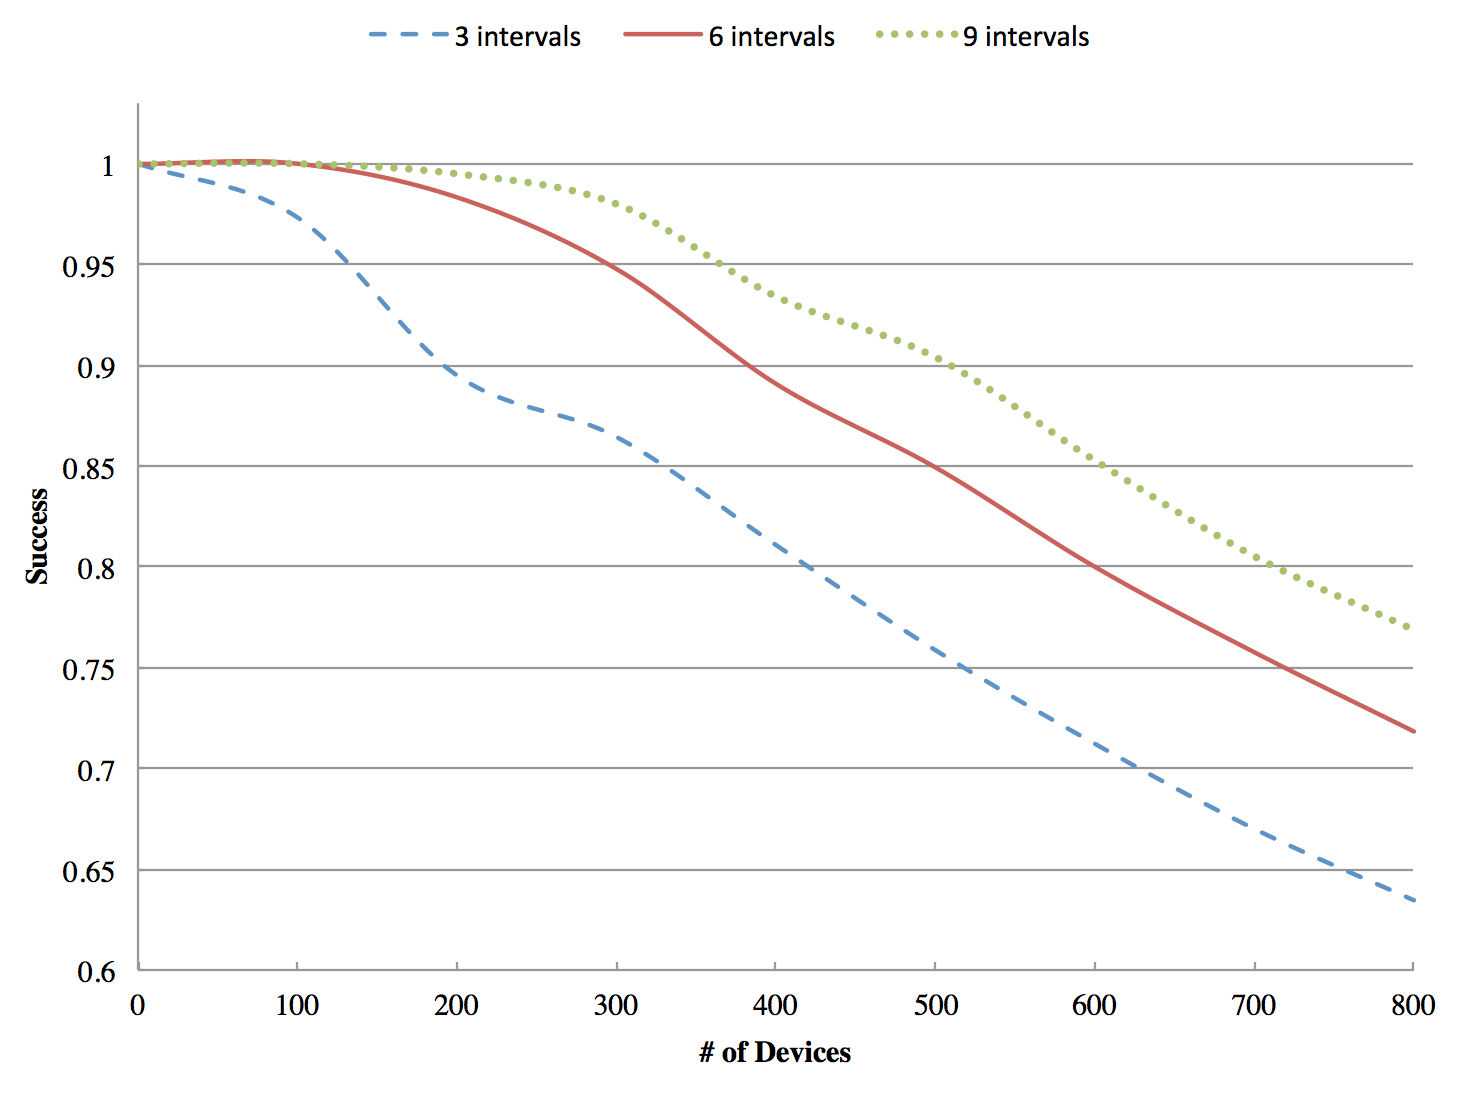
\includegraphics[width=\columnwidth]{figures/square-topo-error.png}
\caption{Transmission success rate across all intervals for square topology, all devices located 1m apart in a grid.}
\label{fig:square-topo-error} \end{figure}

To complete our simulation analysis of BLEATS, we measure the effect of a
classroom topology upon the reliability of transmission at different scales of
device density. The topology follows a two-dimensional square grid with 1 meter
between each device in the topology. The single beacon receiver that records
attendance is located at the center border of the topology, i.e. the "head of
the classroom." Compared to the single-point baseline topology, we observe that
the reliable transmission threshold for this square topology occurs at
a lower numbers of devices. For instance, 100\% reliability is only
feasible for up to 100 devices. This is expected because the distribution of
devices creates more collision points for beacon packets being broadcasted.

Combining the negative effects of moderate WiFi interference, real-world
obstacles, and multipath scenarios with the positive effects of increasing
interval duration and number of scanned intervals suggests that BLEATS is a
feasible CAT system that warrants additional practical study. 




